\documentclass{article}
\usepackage{graphicx}
\title{Background Report to the Translation Website Project of Team O}
\author{Stephen Hayton
	\\Alasdair Campbell
	\\Wei Zhang
	\\Andrei Mustata
	\\Paul Moore}
\date{11th January 2012}

\begin{document}

\maketitle

The purpose of this document is to serve as an introduction to the Translation Website Project of Team O. It aims to provide a useful summary of the project description, the early design decisions involved and the difficulties we've faced in making such decisions. It will also provide detail of how we have so far drawn on knowledge gained in past Computing Science modules, in order to create a useable, competitive website.\\
\\
To briefly summarise our task at hand: we are to develop a website for a free-lance translator. It should allow users to upload documents, request one of the available languages to translate to, and submit a request for translation. Our client should then be able to review those submitted documents and send a quote to the user for the job to be translated. The user should then be able to pay for the job(s) via Paypal, and then receive their translated document after a period of time. Additional required features of the website will be discussed later.\\
\\
An essential part of our requirements gathering process was the first meeting with our client, Joelle Cimatche. Our team had been forewarned by our supervisor that the client was not very "technically minded", so we tried our best to prepare questions that did not assume she had much experience with a computer. At the meeting, the client explained she had a very basic understanding of word processing applications and the Internet, and not much else. This presented us with an additional challenge. We couldn't simply relay technical jargon to the client and expect her to provide useful feedback. Not only that, our team would have to create a very easy-to-use admin end to the website that she could learn quickly. As we advanced the development of the website, we would have to be very clear and straightforward when updating her on our progress. The figure below illustrates this challenge we have:\\ It is basically the "adoption rate" for a percentage of users of new technologies. In otherwords, how quickly users can say they understand a new technology after it is first released. It is known as Roger's bell curve. Our client would be at the very end of the spectrum, in the 16\% of users or "Laggards" as described in the graph.\\

\begin{figure}
\begin{center}
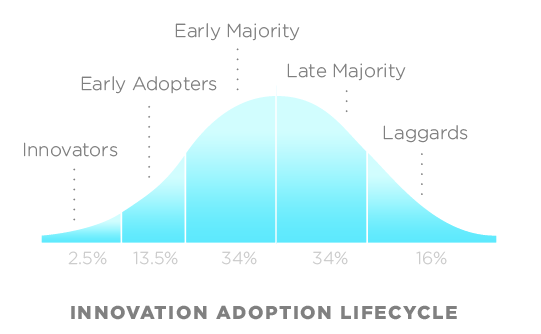
\includegraphics[scale=0.6]{DiffusionOfInnovation}
\caption{Roger's bell curve, source: http://en.wikipedia.org/wiki/File:DiffusionOfInnovation.png}
\end{center}
\end{figure}

As software developers naturally would when creating anything else from scratch, our team looked for similar websites already in existence. We did not try to re-invent the wheel. Instead, we identified common useful features of each, features that were not so useful, and listed some we thought could be useful but simply did not exist in any of the sites we examined. One recurring theme we noticed in a majority of similar translation websites was that the home page was very cluttered. In other words, the process that the user had to follow to obtain some translation of a document was not extremely clear. Instead, they were met with various registration options, other services and annoying advertisements. From previous modules in our degree, namely IM2 and IS3, our team had experience of applying Jakob Nielsen's heuristics to obtain a successful user interface. We wanted to develop the idea that our website would display the minimal amount of information to a user by dividing the registration, document upload and language selection to a single page, 3 step process. Our interface would then fall in line with the principle that user interfaces should have aesthetic and minimalist design. \footnote{http://www.useit.com/papers/heuristic/heuristic\_list.html} We believe this is an extremely important aspect of any modern website based on the way that users make a decision of whether or not to use the services offered by the website. For example, imagine a user enters a Google search for "Translation service" and clicks our website in the results page. If the page they are met with looks too complicated or confusing in nature, the user simply clicks "Back" on their web browser, and goes to the next appropriate web page. If however the website looks clean, simple and easy to use, the user would be more inclined to use the website properly. We believe that our 3-step process found on the home page encourages anyone that requires a translation service for the provided languages to at least try for a quote, if not go through with the whole process.	
\end{document}
